\section{Motivation}
\subsection{Superlight Clients}

Given an honestly adopted chain, consensus security is based on the premise that
it is difficult to create a competing chain which deviates significantly and has
more proof-of-work than the existing honestly adopted chain. To determine which
financial history is the valid one, a \emph{verifier} node booting for the first
time into the network, connects anew to multiple \emph{provers}, at least one of
which is assumed to be honest. The verifier then downloads all available
blockchains from its peers and adopts the longest one. The verifier must choose
the chain that respects the protocol rules and corresponds to the most
proof-of-work. In order to do that, the proof-of-work of every block in the
chain must be presented and verified.

\begin{figure}[tb]%{{{
  \centering
  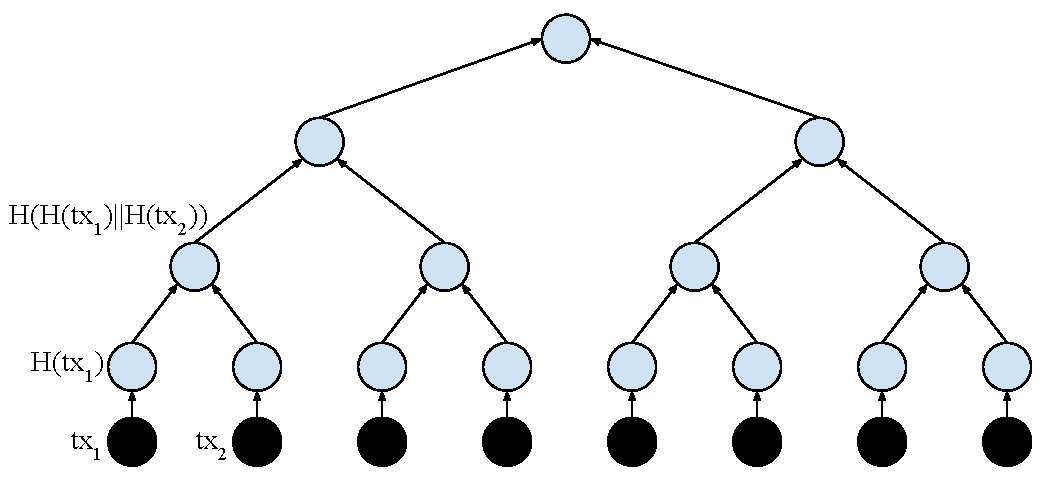
\includegraphics[width=0.9 \textwidth]{chapters/introduction/figures/merkle-tree.pdf}
  \caption{
    A Merkle Tree of transactions making use of a cryptographicallys secure hash
    function $H$. Black nodes indicate raw transactions.
    Lightly shaded nodes indicate hashes. The root is shown at the top.
  }
  \label{fig.merkle}
\end{figure}%}}}

Nodes on the blockchain that maintain the whole history of transactions and
chain are known as \emph{full nodes}. Typically, miners are full nodes, but some
non-mining nodes are also full nodes.
Proof-of-work blockchain clients such as mobile wallets today are based on the
Simplified Payment Verifications (SPV) protocol, which was described in the
original Bitcoin paper~\cite{bitcoin}, and allows them to sychronize with the
network by downloading only block \emph{headers} and not the entire blockchain with
transactions. However, such initial synchronization still requires receiving all
the block headers.

Instead of having each block contain all of its
transactions and performing proof-of-work on it, transactions are first hashed
into a special structure known as a Merkle Tree. A Merkle Tree of a transaction
sequence $\overline{x}$ is structured as illustrated in Figure~\ref{fig.merkle}. Using a cryptographically
secure hash function $H$, each transaction is hashed to obtain its transaction
\emph{id}. Subsequently, each two ids are concatenated together and hashed again
to obtain their parent. These parents are again concatenated and hashed
together to obtain \emph{their} parent, until we arrive at a single \emph{root}
node $x$ which contains a hash representation of every transaction in
$\overline{x}$. The proof-of-work of the block is then computed by finding a
$\textsf{nonce}$ such that $H(x \concat \textsf{nonce} \concat h') \leq T$. The
transactions $\overline{x}$ are known as the \emph{block content}, while the
portion $x \concat \textsf{nonce} \concat h'$ which is hashed for proof-of-work
purposes is known as the \emph{header}.

This chain $\chain$ of block headers grows linearly in time. To put the problem
in perspective and motivate the question, at the time of writing, Ethereum's
blockchain (as measured by the amount of data that needs to be downloaded to
synchronize a full node) is currently more than $250$GB, and the size of block
headers is $4.6$GB. The latter amount is currently too large for a user-friendly
mobile wallet.

The problem we concern ourselves with is whether it is possible to optimize this
protocol, achieving communication $o(|\chain|)$. We study the question of
whether better protocols exist and in particular if downloading fewer block
headers is sufficient to securely synchronize with the rest of the blockchain
network. Our requirement is that the system remains decentralized and that
useful facts about the blockchain (such as the Merkle root of current account
balances in Ethereum) can be deduced from the downloaded data. This means that
we don't want to utilize techniques such as checkpointing (in which the verifier
software is patched by its trusted developer to include a later block as
a \emph{neon genesis} replacement to the genesis block) or trusting a server to
give us the correct blockchain.

Our setting is as follows. A \emph{superlight} verifier wakes up having only the
first block of the blockchain, the genesis block. In the meantime, the
blockchain has grown and contains many blocks. The verifier wishes to know
whether a transaction is confirmed to decide if a payment has been made. It
connects to multiple other \emph{full nodes}, that we term \emph{verifiers}
throughout this work, who maintain the whole blockchain. At least one connection
will be to an \emph{honest node}. All the provers send some claims to the
verifier, some claiming that the transaction is confirmed, while others that it
is not. The goal of the verifier is to decide which of these claims is true. The
claims are accompanied by \emph{evidence} to illustrate them, but must be short
in length so that the client can synchronize quickly. In particular, we aim for
exponentially shorter messages $\bigO(polylog(|\chain|))$ instead of the
standard $\bigO(|\chain|)$ than an SPV node requires. These superlight nodes are
useful when a client such as a mobile wallet wishes to synchronize with the
network quickly. Other facts beyond transaction inclusion, such as account
balances, are also useful to prove.

The question the verifier is trying to answer is not simply whether the
transaction has been included in \emph{some} valid block, but whether that block
belongs to the longest chain. For the proof-of-work case, this chain corresponds
to the chain containing the most proof-of-work that respects the protocol rules
(such as the occasional recalculation of the target $T$). For proof-of-stake,
this chain corresponds to the longest chain which has valid signatures by the
majority of the stakeholders at each point in time, keeping in mind that stake
is shifting from epoch to epoch.

\todo{continuity}

\subsection{Interoperability}
Since the invention of Bitcoin in 2009, numerous other cryptocurrencies have
followed, improving upon Bitcoin on several aspects. The most prolific of these
is \emph{Ethereum}~\cite{buterin}, which introduces the concept of \emph{smart
contracts}. These Turing-complete programs enable developers to define complex
conditions which must be satisfied to spend money, beyond the simple signatures
that Bitcoin allows as conditions for spending. They are programmed in
specialized programming languages such as Solidity and run on top of the
Ethereum Virtual Machine~\cite{wood}. Each contract is a sovereign entity that
can own money and define the rules under which this money can be spent. These
contracts execute autonomously. Their correct execution is verified by miners on
the network, in a similar way that signatures are verified in Bitcoin's case.

Other cryptocurrencies that include significant contributions and
experimentation are \emph{Litecoin}~\cite{litecoin} which aims to be more
egalitarian~\cite{egalitarianism}; \emph{Monero}~\cite{cryptonote} and
\emph{ZCash}~\cite{zerocoin,zcash}, which improve upon the generally
poor~\cite{fistful,quantitative-bitcoin-analysis,tumblebit} privacy of
Bitcoin; \emph{Namecoin}~\cite{namecoin} which was a first attempt at creating a
decentralized DNS alternative; \emph{Dogecoin}~\cite{dogecoin}, which experiments with
inflationary economics in contrast to Bitcoin's deflationary nature;
\emph{Bitcoin Cash}~\cite{btcVSbch}, which experiments with larger block sizes; and
\emph{Cardano}~\cite{ouroboros}, which uses proof-of-stake instead of proof-of-work.

It is possible to \emph{trade} one coin for the other. For example, if one
wishes to exchange Bitcoin for Ethereum, they need to find a counterparty who
wishes to exchange Ethereum for Bitcoin (this is generally easy to do through
centralized services). However, each of these blockchain systems remains
isolated. The concept of a \emph{cryptocurrency} and its respective \emph{chain}
remains intertwined: A Bitcoin lives in the Bitcoin chain, while an Ether lives
in the Ethereum chain. The \emph{interoperability} problem pertains to the
ability to move a cryptocurrency from its native chain to a remote chain,
a one-way peg\index{One-way Peg}, and then back, a two-way
peg\index{Two-way Peg}. If Bitcoin and Ethereum were interoperating, it would be
possible to move one Bitcoin from the Bitcoin chain to the Ethereum chain and
back. In a properly interoperating system, the Bitcoin would retain its nature
during its lifespan within the Ethereum chain. For example, it would maintain
the same exchange rate against other currencies as a Bitcoin living in the
Bitcoin chain. While on the Ethereum chain, it would also enjoy the benefits of
the Ethereum ecosystem. For example, it would make itself subject to smart
contracts.

\todo{continuity here}

The smart contracts are confined to access data only within the blockchain
itself, such as data maintained within the state of the smart contract itself.
Access to external data
requires a trusted third party or group thereof to vouch for the data
validity~\cite{towncrier}.

\todo{continuity here}

Sidechains~\cite{sidechains} are a mechanism for cross-chain communication in
blockchains. They allow smart contracts on one blockchain to receive and
react to \textit{events} taking place on another blockchain without the need
of trusted parties. Despite their widely agreed usefulness
there exist no constructions that are decentralised and efficient at the same
time.

\todo{continuity}

While enjoying wide adoption,
there  are several fundamental open questions remaining to be resolved
that include (i)
         Interoperability:
           How can different blockchains interoperate and exchange
           assets or other data?
(ii)  Scalability:
           How can blockchain protocols scale, especially proportionally to the number of           participating nodes?
(iii)
         Upgradability:
           How can a deployed blockchain protocol codebase evolve to support a new
           functionality, or correct an implementation problem?

The conditions used to validate transactions %for each node of the system
depend on local blockchain events according to the view of each node and they
typically cannot be dependent on other blockchain sessions. Being
able to perform operations across blockchains, for instance from a main blockchain
such as Bitcoin to a ``sidechain'' that has some enhanced functionality, has been
frequently considered  a fundamental technology enabler in the blockchain space.\footnote{See
e.g., \url{https://blockstream.com/technology/} and \cite{sidechains}.  }

\todo{continuity}

Sidechains, introduced in \cite{sidechains},  are a
way for multiple blockchains to communicate with each other and have one react
to events in the other. Sidechains can exist in two forms. In the first case, they are simply a mechanism for two
existing \textit{stand-alone blockchains} to communicate, in which case any of
the two blockchains can be the sidechain of the other and they are treated as
equals. In the second case, the
sidechain can be a ``child'' of an existing blockchain, the \textit{mainchain},
in that its genesis block, the first block of the blockchain, is somehow seeded
from the parent blockchain and the child blockchain is meant to depend on the
parent blockchain, at least during an initial bootstrapping stage.

A sidechain system can choose to enable certain types of interactions between
the participating block\-chains. The most basic interaction
is the transfer of assets from
one blockchain to another. In this application, the nature of the asset
transferred is retained in that it is not transformed into a different class of
asset (this is in contrast to a related but different concept of \emph{atomic
swaps}).
As such, it maintains its value and may also be transferred back.
The ability to move assets back and
forth between two chains is sometimes referred to as a \textit{2-way peg}. Provided
the two chains are both secure as individual blockchains, a secure
sidechain protocol construction allows this security to be carried on to
cross-chain transfers.

A secure sidechain system could be of a great value vis-\`a-vis all three
of the pressing open questions in blockchain systems mentioned above. Specifically:

%\noindent
{\em Interoperability.} There are currently hundreds of
    cryptocurrencies deployed in production. Transferring assets between
    different chains requires transacting with intermediaries (such as exchanges). Furthermore,
    there is no way to securely interface with another blockchain to react to
    events occurring within it. Enabling sidechains allows
    blockchains of different nature to communicate, including interfacing with
    the legacy banking system which can be made available through the use of
    a private ledger.

%\noindent
{\em   Scalability.} While sidechains were not originally proposed for
    scalability purposes, they can be used to off-load the load of a blockchain
    in terms of transactions processed. As long as 2-way pegs are enabled, a
    particular sidechain can offer specialization by, e.g., industry, in order
    to avoid requiring the mainchain to handle all the transactions occurring
    within a particular economic sector. This provides a straightforward way to
    ``shard'' blockchains, cf. \cite{sharding,omniledger,rapidchain}.

%\noindent
{\em Upgradability.} A child sidechain can be created from a parent
    mainchain as a means of exploring a new feature, e.g., in the scripting language, or
    the consensus mechanism
    without requiring a soft, hard, or velvet fork~\cite{nipopows,velvet}. The
    sidechain does not need to maintain its own separate currency, as value can
    be moved between the sidechain and the mainchain at will. If the feature of
    the sidechain proves to be popular, the mainchain can eventually be
    abandoned by moving all assets to the sidechain, which can become the new
    mainchain.

Given the benefits listed above for distributed ledgers, there is a pressing
need to address the question of sidechain security and feasibility, which so far, perhaps surprisingly, has not received any proper formal treatment.
